\documentclass[11pt,a4paper]{article}
\usepackage[margin=2.3cm]{geometry}
\usepackage{graphicx,booktabs,amsmath,amssymb,hyperref,caption,subcaption,array}
\usepackage[T1]{fontenc}\usepackage{lmodern}
\hypersetup{colorlinks=true,linkcolor=black,urlcolor=blue}
\emergencystretch=3em\setlength{\parskip}{0.5em}\setlength{\parindent}{0pt}
\title{CS 631 Project --- Index Selection on PostgreSQL: Reproducing the Kossmann et al.\ Evaluation and Adding Budget-Aware Tuning (Wii, Esc)}
\author{Arijit Mandal \and Rameez Wahid \and Harshvardhan Shinde \and Prathamesh Thakur}
\date{25 November 2026}
\begin{document}
\maketitle

\begin{abstract}
We reproduce the TPC-H (scale factor 10) experiment of Kossmann et al.\ (PVLDB 13(11), 2020) on PostgreSQL 18.7 with the authors' platform, and extend it with budget-aware index tuning: a two-phase greedy tuner with the call-skipping mechanism Wii (Wang et al., SIGMOD 2024) and the early-stopping checker Esc (Wang et al., PVLDB 2025), both implemented by us from the papers because no code was available. The original study's picture is reproduced in shape: the same cost cliff, a cluster of near-equal algorithms, and the same ordering of run times; the cliff sits at a smaller budget, CoPhy ends about 4 points better, and run times are 2--10$\times$ lower. Judged by the optimizer's estimates, Wii finds indexes with 96\% of the improvement of the unrestricted tuner using 14\% of its what-if calls (32.7\% against 33.9\% improvement, 430 against 3\,040 calls; four statistics draws), and against the original eight algorithms at 10\,GB the tuner with Wii reaches 68.3\% relative cost with 430 calls, where CoPhy reaches 66.3\% with 23\,066. Esc saves 5--28\% of the calls in the storage-limited setting, with a storage-aware bound that we added (on synthetic data Esc never stopped without it; we did not measure its effect on TPC-H), and it adds nothing on top of Wii. These results rest on estimates. When we built the indexes chosen at a 5\,GB budget and ran the queries, only the plain two-phase greedy was faster than no indexes (by 35\%); Extend, Relaxation, Wii, Esc and Wii~+~Esc were 3--40\% slower, although all six were estimated to improve the workload by 26--29\%. The estimated quality of an algorithm therefore does not show how good its indexes are in practice, and this limits every comparison in the report.
\end{abstract}

\section{Introduction}
Index selection algorithms choose indexes for a workload under a storage or count budget, usually by asking the optimizer for the cost of the workload under hypothetical (what-if) indexes. Kossmann et al.\ compared eight algorithms (Extend, Relaxation, DTA, CoPhy, DB2Advis, AutoAdmin, Drop, Dexter) on several workloads and DBMSs. The project had three objectives:
\begin{enumerate}
\item \textbf{Reproduce} the TPC-H SF10 evaluation on a current PostgreSQL (Section~\ref{sec:repro}).
\item \textbf{Extend} it with budget-aware tuning, Wii and Esc, and compare them with the original eight (Sections~\ref{sec:setup}--\ref{sec:compare}).
\item \textbf{Execute} the selected indexes and time the queries, instead of relying on estimates (Section~\ref{sec:exec}).
\end{enumerate}
\textbf{Contributions.} A reproduction with three repetitions per point; an implementation of a budget-aware two-phase greedy with Wii, Esc-B and their evaluation; three additions of our own to Esc (the storage budget in the simulated greedy, a storage-aware upper bound, and an optional clamp that is a heuristic); and a real-execution check that shows the limits of estimate-based comparisons. What is \emph{not} done is listed in Section~\ref{sec:limits}.

\section{Reproduction of the original evaluation}\label{sec:repro}
\textbf{Setup.} TPC-H SF10, 19 queries (2, 17 and 20 excluded, as in the paper). The metric is the relative workload cost: the optimizer's estimate for the workload with the selected hypothetical indexes divided by the estimate without indexes. All eight algorithms ran with the repository configuration \texttt{tpch\_sf10\_paper.json}: storage-budget algorithms at 16 budgets from 250 to 15\,000\,MB, AutoAdmin and Drop at 1--13 indexes, Dexter at 5 thresholds; every point three times (112 parameter points). Differences from the paper: PostgreSQL 18.7 instead of 12.1, HypoPG 1.4.5, Dexter 0.6.3, CoPhy solved with Gurobi 13 through PuLP 3 and index width 3 in the main run (the paper states 2), and different hardware.

\begin{figure}[h]\centering
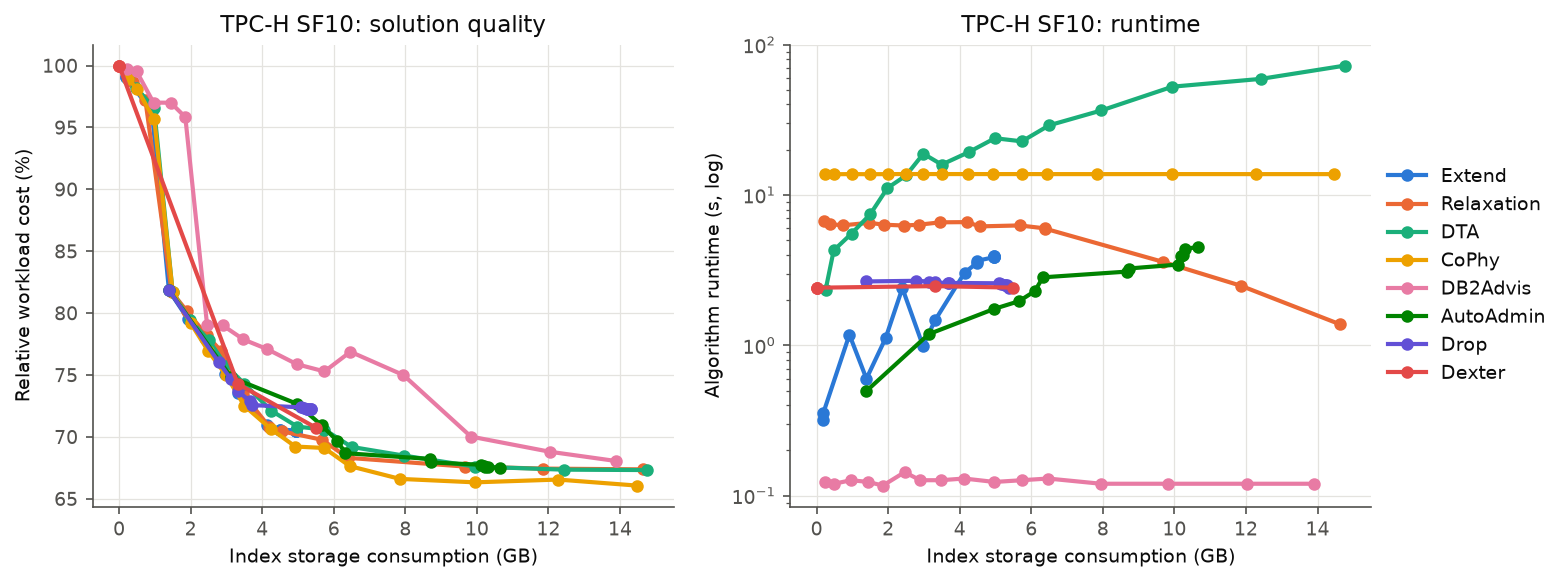
\includegraphics[width=\textwidth]{tpch_sf10_reproduction.png}
\caption{TPC-H SF10: relative workload cost (left) and algorithm run time (right, log scale), means of three repetitions.}\label{fig:repro}
\end{figure}

\textbf{What reproduces.} All storage-budget algorithms except DB2Advis follow almost the same curve. Nothing helps below about 1.4\,GB; once the budget admits one large index on \texttt{lineitem.l\_orderkey}, the cost drops from about 96\% to 82\% for every algorithm. Beyond 6\,GB, Relaxation, DTA, AutoAdmin and CoPhy end within 67.3--67.7\% (CoPhy re-run at width 2), Extend at 70.5\%. DB2Advis is fast (0.1\,s) but needs more space for the same quality. The ordering of run times (DB2Advis $\ll$ Extend, Drop, Dexter $<$ Relaxation $<$ CoPhy, DTA growing with the budget) agrees with the paper, and so does Dexter's operating point (70.7\% at about 5.4\,GB).

\textbf{What differs.} (1) The cliff is at about 1.4\,GB instead of the paper's 2\,GB; HypoPG's size estimate for the large index is clearly smaller, and we did not isolate the cause (PostgreSQL version and the newer estimator are candidates). (2) CoPhy is among the best here, but not in the paper. Re-running it at width 2 removes only about 1 point; about 4 points remain unexplained. (3) Absolute run times are 2--10$\times$ lower with the same shapes; we attribute this to newer hardware and software without having tested it, and we compare orderings, not seconds. Paper values were read off its figures (accuracy about $\pm$1--2 points).

\textbf{Variability.} \texttt{ANALYZE} samples rows randomly, so each repetition sees different statistics. The largest spread over repetitions is 3.15 points for DTA, 2.51 for CoPhy, 1.70 for Relaxation, 1.57 for DB2Advis, 1.09 for AutoAdmin, 1.07 for Extend, 0.39 for Drop and 0.29 for Dexter. Differences of one to two points between Relaxation, DTA, AutoAdmin and CoPhy at large budgets are within noise, and we do not rank them.

\section{Budget-aware tuning: setup}\label{sec:setup}
\textbf{Tuner.} The project's platform now contains a two-phase greedy algorithm (per-query greedy search, then greedy over the union of the selected indexes) running behind a cost oracle that counts and limits what-if calls. The oracle has four modes: \emph{none} (every cost question is answered by a what-if call until the budget is spent, after which the cheapest known cost of a subset of the configuration is used), \emph{Wii}, \emph{Wii + coverage} (a refinement of Wii's bounds) and \emph{random} (skips a call with fixed probability; used as a control). Wii skips a call when the lower bound $L$ on the query's cost under a configuration is within a factor $\alpha$ of the upper bound $U$ (the cheapest known cost of any subset), i.e.\ $L/U\ge\alpha$, and uses $U$ instead. The initial calls (no-index cost, and the cost with all candidates for Wii) count against the budget.

\textbf{Workload and environment.} TPC-H, SF10, 19 queries (2, 17 and 20 excluded, as in the platform's baseline experiments). PostgreSQL 18.7, HypoPG 1.4.5, all planner settings at their defaults (\texttt{max\_parallel\_workers\_per\_gather}=2, \texttt{work\_mem}=4\,MB, \texttt{shared\_buffers}=128\,MB, \texttt{random\_page\_cost}=4, \texttt{effective\_cache\_size}=4\,GB). Index width up to 2; the constraint is the number of indexes $K\in\{10,20\}$ with no storage limit, except in Sections~\ref{sec:compare} and~\ref{sec:storage}, which use storage budgets with $K=100$. Each statistics draw is a fresh \texttt{ANALYZE}; we report four draws (no-index workload cost 42\,621\,151 to 42\,660\,191), of which the first (42\,625\,951) was used for the assumption and gap experiments and for nothing else; Section~\ref{sec:compare} uses its own runs.

\textbf{Metric.} Improvement $=1-\text{cost}(\text{indexes})/\text{cost}(\emptyset)$, with the cost of the final configuration obtained by fresh what-if calls for every query (not from the tuner's own, possibly derived, numbers). ``Calls'' are what-if calls issued by the oracle; repeated questions and indexes irrelevant to a query are not counted.

\section{Wii: results}
\subsection{Quality against call budget}
\begin{figure}[h]\centering
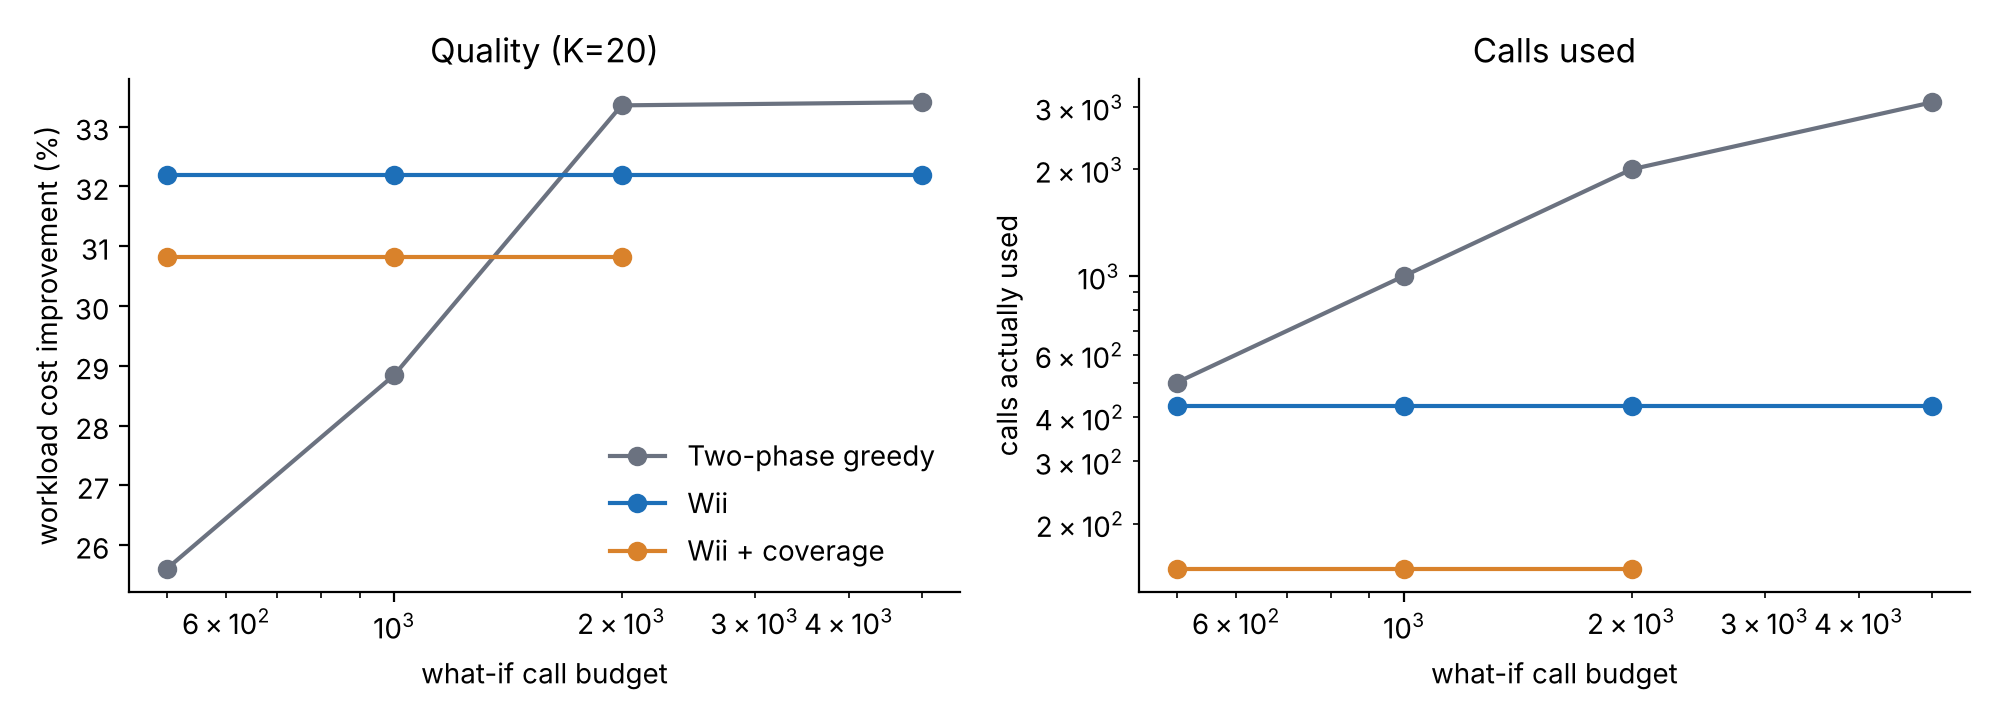
\includegraphics[width=\textwidth]{fig_budget.png}
\caption{Improvement (left) and what-if calls actually used (right) for $K=20$. Wii (alpha 0.9) always needs the same number of calls (429 in this draw, 429--437 over four draws) and wii+coverage about 149, so their curves are flat; the baseline is limited by the budget. Figures show the first statistics draw.}\label{fig:budget}
\end{figure}

\begin{table}[h]\centering\small
\begin{tabular}{lrrrr}\toprule
Budget $B$ & Baseline & Wii ($\alpha=0.9$) & Wii + coverage & Baseline calls\\\midrule
500 & 25.57\% & 32.71\% (433 calls) & 31.23\% (149) & 500\\
1000 & 29.37\% & 32.71\% & 31.23\% & 1000\\
2000 & 33.88\% & 32.71\% & 31.23\% & 2000\\
5000 (not binding) & 33.95\% & 32.71\% & -- & 3036\\\bottomrule
\end{tabular}
\caption{TPC-H SF10, $K=20$, means over four statistics draws. Ranges over the draws: baseline 25.48--25.62, 28.83--29.97, 33.33--34.50 and 33.39--34.58\%; Wii 32.18--33.29\%; coverage 30.80--31.70\%. For $K=10$ the Wii rows are identical and the baseline gives 25.57, 29.37, 33.23 and 33.52\% (2\,723 calls at $B=5000$).}\label{tab:main}
\end{table}

Wii is 6.6--7.7 points better than the baseline at $B=500$ and 3.3--3.4 points better at $B=1000$, in each of the four draws. At $B=2000$ the baseline, now with enough calls, overtakes it by 1.2 points in every draw. The absolute values move by about 1 point between draws, but these paired differences hardly move. Wii never uses more than 437 calls, so the larger budgets of this sweep do not constrain it: within one draw the four Wii entries in Table~\ref{tab:main} are one and the same run. A sweep of smaller budgets would be needed to see where Wii itself starts to degrade; the 38 initial calls set a lower limit.

\subsection{The role of alpha}
\begin{figure}[h]\centering
\begin{subfigure}{0.48\textwidth}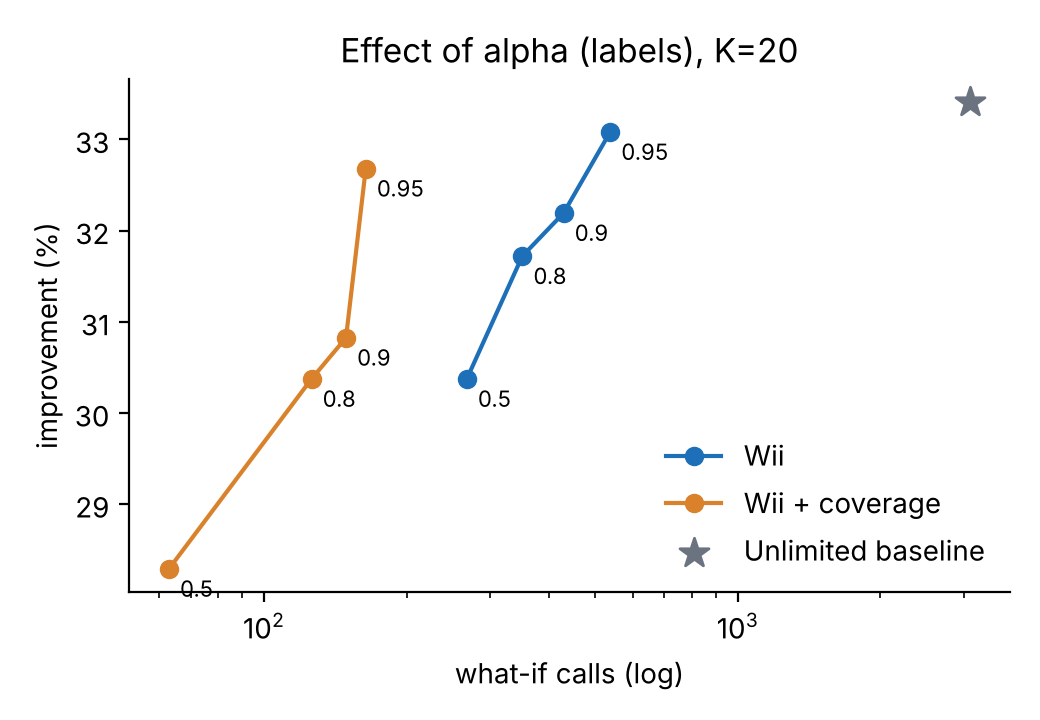
\includegraphics[width=\textwidth]{fig_alpha.png}\caption{Improvement against calls for different $\alpha$.}\end{subfigure}\hfill
\begin{subfigure}{0.48\textwidth}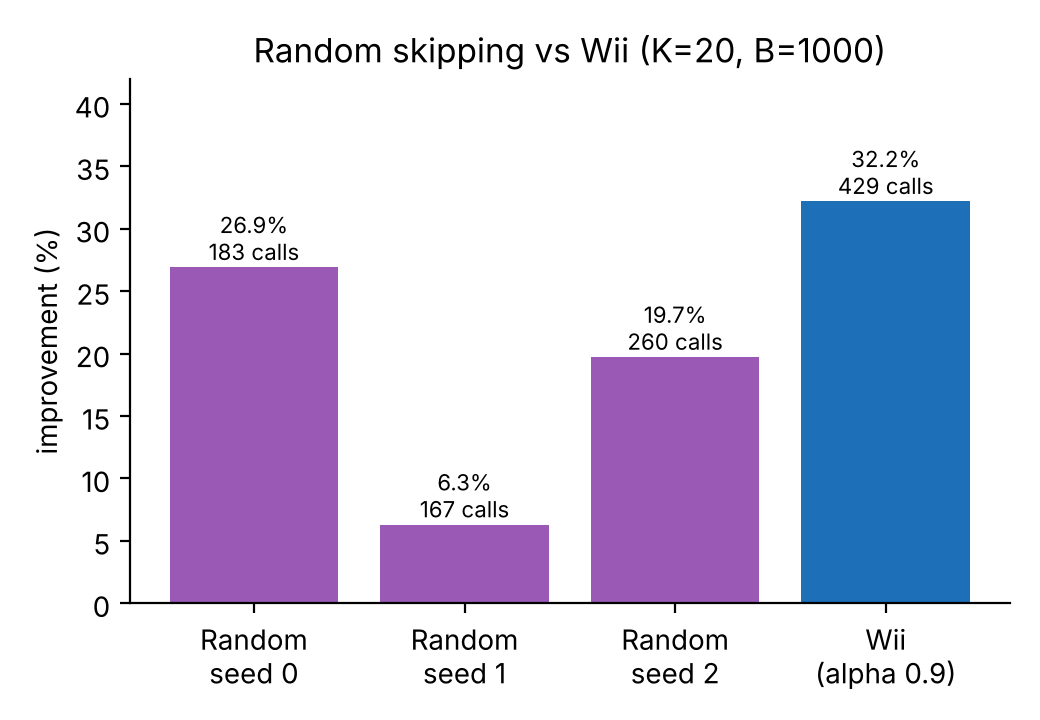
\includegraphics[width=\textwidth]{fig_random.png}\caption{Random skipping against Wii.}\end{subfigure}
\caption{Left: higher $\alpha$ skips fewer calls and gives better indexes. Right: random skipping at probability 0.9 with three seeds, against Wii.}\label{fig:alpha}
\end{figure}

\begin{table}[h]\centering\small
\begin{tabular}{lrrr}\toprule
$\alpha$ & Wii improvement (calls) & Wii + coverage (calls) & Wii quality vs.\ unlimited\\\midrule
0.5 & 30.77\% (268) & 29.73\% (66) & 90.6\%\\
0.8 & 32.12\% (351) & 30.78\% (127) & 94.6\%\\
0.9 & 32.71\% (433) & 31.23\% (149) & 96.3\%\\
0.95 & 33.59\% (538) & 33.04\% (170) & 98.9\%\\\bottomrule
\end{tabular}
\caption{Alpha sweep ($K=20$, $B=1000$), means over four draws (spread 0.5--1.2 points, up to 3 points for coverage at $\alpha=0.5$); the unlimited baseline reaches 33.95\% with about 3\,036 calls.}\label{tab:alpha}
\end{table}

With $\alpha=0.95$ Wii reaches 99\% of the unlimited baseline's improvement with 538 calls (18\% of 3\,036). The coverage refinement uses fewer calls at the same $\alpha$ but gives lower quality in every row and every draw on this workload.

\textbf{Random skipping.} Skipping 90\% of calls at random gives 23.0\%, 7.0\% and 20.1\% improvement for three seeds (means over four draws; the first seed ranges from 19.0 to 26.9\% between draws), using 149--260 calls, while Wii gets 32.7\% with 433. Which calls are skipped matters: Wii's bounds pick calls that carry little information, random skipping does not. The large spread between seeds (7--27\%) also means a single random seed would be misleading.

\subsection{Why skipping is safe: derived against real costs}\label{sec:gaps}
\begin{figure}[h]\centering
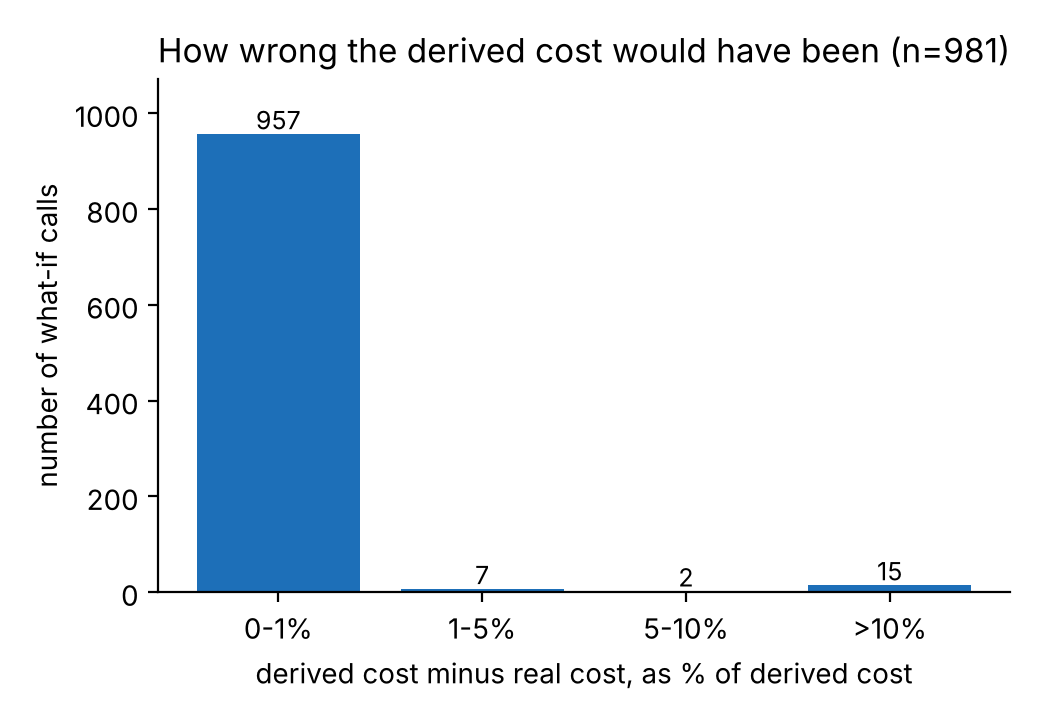
\includegraphics[width=0.55\textwidth]{fig_gaps.png}
\caption{For every real what-if call of a budgeted baseline run ($K=20$, $B=1000$), the error the derived cost would have had.}\label{fig:gaps}
\end{figure}
In 957 of 981 calls (97.6\%) the cost derived from already-known configurations is within 1\% of the real cost; only 15 calls (1.5\%) are off by more than 10\%. Most what-if calls of the baseline are therefore redundant, which is what Wii exploits.

\subsection{Assumptions of the cost model}\label{sec:assump}
Wii's bounds rest on monotonicity (adding an index does not increase the cost) and submodularity (the benefit of an index does not grow when other indexes are present). Using the best single index of each query paired with each other candidate (643 pairs over 19 queries), PostgreSQL's cost model violates monotonicity in 3 pairs (0.5\%) and submodularity in 9 pairs (1.4\%). The worst monotonicity violation is query~8, where adding an index raised the estimated cost by 19\%. The violations are rare, which is consistent with Wii's small quality loss, but they mean the bounds are not guaranteed.

\section{Esc: early stopping}\label{sec:esc}
\textbf{Implementation.} Esc-B (the variant without index interaction) is checked at the start of each greedy step of the second phase. It stops when $\eta_U-\eta_L\le\epsilon$: $\eta_L$ is the improvement of a simulated greedy completion that uses derived costs only; $\eta_U$ is Eq.~10 of the paper, the $K$ largest workload-level marginal-improvement bounds summed. On stopping, the simulated completion is returned. Esc-I, the generic rate-based filter and the MCTS variants are not implemented. A second, optional variant (``clamped'', our addition) additionally caps $\eta_U$ at the improvement obtained with all candidate indexes at once.

\begin{table}[h]\centering\small
\begin{tabular}{llrrrr}\toprule
$K$ & Variant & $\epsilon$ & Calls saved & Improvement lost & Guarantee\\\midrule
20 & plain Esc-B & 1--2\% & 16.9--19.8\% & 0.00 pts & yes\\
20 & plain Esc-B & 5--10\% & 24.3--27.8\% & 0.00 pts & yes\\
10 & plain Esc-B & 1--2\% & 8.9--9.9\% & 0.04 pts & yes\\
10 & plain Esc-B & 5--10\% & 17.1--18.8\% & 0.04--0.19 pts & yes\\
20 & clamped & 1--10\% & 33.3--37.5\% & 0.04--0.05 pts & no\\
10 & clamped & 1\% & 24.3--26.7\% & 0.13 pts & no\\
10 & clamped & 2--10\% & 27.0--29.8\% & 0.59--0.63 pts & no\\
20 & Wii + plain & any & 0.0\% & 0.00 pts & yes\\
20 & Wii + clamped & 1--10\% & 7.4--7.5\% & 0.00 pts & no\\
10 & Wii + clamped & 1\% & 1.9--2.1\% & 0.00--0.02 pts & no\\
10 & Wii + clamped & 2--10\% & 7.4--7.5\% & 0.09--0.11 pts & no\\\bottomrule
\end{tabular}
\caption{Esc on TPC-H SF10: calls saved and improvement lost relative to the same run that never stops (about 3\,000 calls without Wii and 430 with Wii at $K=20$). Ranges are over independent statistics draws (three for plain Esc-B, two for the clamped variants; no-index cost 42.59--42.69M).}\label{tab:esc}
\end{table}

\textbf{Without Wii.} Plain Esc-B saves 17--28\% of the calls at $K=20$ and 9--19\% at $K=10$ across three statistics draws, with at most 0.19 points of quality lost (none at $K=20$). The actual loss is far below the tolerated $\epsilon$ because the bound is loose (a gap of 2.6--3.0 points at the first check). Stopping points are coarse: a check happens only at Phase-2 steps, and for $\epsilon\gtrsim3\%$ the first check already passes. The check costs 0.03--0.08\,s.

\textbf{With Wii.} The plain checker never stops (430 calls in every run). Wii skips the calls that would give exact costs for the bound, so $\eta_U$ stays at 0.544 against $\eta_L=0.333$ after Phase~1 (from an earlier draw). Only about 36 of the calls come after Phase~1, so even a perfect checker could save at most about 8\%.

\textbf{Storage of the stopped configuration.} In all three draws the configuration returned by plain Esc-B at $K=20$ costs the same as the never-stopping run's (to 0.01 points) but swaps 2--3 of its 20 indexes for others, and takes 1.4--2.0\,GB (13--19\%) more space (10.3 against 12.3\,GB in the third draw). The simulated completion only sees derived costs, in which the swapped indexes are interchangeable, so it can pick larger ones. The paper's early stopping is about calls, so this is not a flaw in the bound, but it matters when storage is limited, and Esc would then need a storage-aware tie-break.

\textbf{The clamp is a heuristic.} With it, 7.4--7.5\% of calls are saved with Wii and 33--38\% without (two draws). But the clamp assumes that adding indexes never raises the estimated cost, and PostgreSQL does not guarantee that (see above): at $K=20$ without Wii the checker stopped with $\eta_L=0.3203$ above the clamped $\eta_U=0.3161$ (first draw), and in the second draw the violation counter registered one violation in each clamped $K=20$ run without Wii and none in any other run. The bound is then raised to $\eta_L$ and the event counted, so the clamped checker keeps no guarantee. In our runs the actual loss stayed below $\epsilon$ (at most 0.59 points, at $K=10$), but this is an observation, not a bound.

\subsection{Storage-limited setting}\label{sec:storage}
Under a storage budget two things change. (1) The simulated greedy that supplies $\eta_L$, and whose configuration is returned when Esc stops, ignored the budget, so the returned configuration could exceed it. This was found in review and is fixed: the simulation now obeys \texttt{budget\_MB}. (2) With $K=100$ the count limit never binds, so Eq.~10 sums the best 100 savings without regard to index size and $\eta_U$ stays far above $\eta_L$. We therefore also cap $\eta_U$ by the fractional knapsack bound (best saving per byte first, the last index counted in part); both relaxations are upper bounds, so the smaller is used. This is our addition, not the paper's. On synthetic cost data with a storage budget the count-only bound stopped in 0 of 15 runs and the storage-aware one in 15 of 15; unit tests check that the bound stays above the improvement the search reaches.

\begin{table}[h]\centering\small
\begin{tabular}{rrrrrrr}\toprule
Budget (GB) & Calls, plain & Calls, Esc & Calls saved & Cost \%, plain & Cost \%, Esc & Stopped\\\midrule
0.25 & 573 & 538 & +6.1\% & 98.9 & 98.9 & 3/3\\
1 & 1011 & 906 & +10.4\% & 96.9 & 96.9 & 3/3\\
2 & 1384 & 1214 & +12.3\% & 80.1 & 80.1 & 3/3\\
2.5 & 1685 & 1704 & -1.1\% & 78.8 & 78.8 & 0/3\\
3 & 1747 & 1766 & -1.1\% & 75.7 & 75.7 & 0/3\\
4.25 & 2179 & 1960 & +10.1\% & 71.5 & 70.6 & 3/3\\
6.5 & 2533 & 2147 & +15.2\% & 67.9 & 68.1 & 3/3\\
10 & 2828 & 2184 & +22.8\% & 67.3 & 67.3 & 3/3\\
15 & 3026 & 2184 & +27.8\% & 67.1 & 67.1 & 3/3\\\\\bottomrule
\end{tabular}
\caption{Esc-B ($\epsilon=5\%$) under storage budgets ($K=100$), TPC-H SF10, means over three repetitions. Cost is the relative workload cost. ``Stopped'': repetitions in which Esc stopped before the search ended. A negative saving at 2.5 and 3\,GB is the 19 extra calls Esc needs for the all-candidates costs.}\label{tab:escstorage}
\end{table}

Esc stopped in all three repetitions at 14 of the 16 budgets (not at 2.5 and 3\,GB). The calls saved grow with the budget, from 6\% at 250\,MB to 28\% at 15\,GB, because the plain search keeps spending calls while the improvement has stopped growing. The relative cost is the same as without Esc to within 0.2 points (at 6.5\,GB 68.1 against 67.9\%; at 4.25\,GB and 5.75\,GB it is lower, 70.6 against 71.5\% and 69.8 against 70.5\%). The paper reports about 60\% savings for two-phase greedy on TPC-H with SQL Server; we get at most 28\%. We have not measured how much of the stopping is due to the storage-aware bound on TPC-H; \texttt{configs/tpch\_sf10\_esc\_ablation.json} runs the same sweep with the count-only bound for that check.

Esc saves what-if calls, not wall-clock time, here: a HypoPG what-if call costs only a millisecond or two, and the checker's simulated greedy at $K=100$ costs about as much. Esc's runtime is higher than the plain search at 9 of 16 budgets (for instance 8.4 against 4.1\,s at 8\,GB) and lower at 5 (3.5 against 4.9\,s at 15\,GB). Combined with Wii, Esc stopped only at budgets up to 2\,GB (and in two of three repetitions at 3.5\,GB), and saved at most two calls (407 against 405 at 3.5\,GB); at larger budgets it never stopped.

\section{Comparison with the eight algorithms}\label{sec:compare}
Greedy, Wii, Esc and Wii~+~Esc were run through the platform like the original eight (\texttt{configs/tpch\_sf10\_new\_algos.json}), at the same 16 storage budgets with $K=100$, so the storage budget is the binding constraint, as for the original algorithms. Both sets of runs have three repetitions, each with its own statistics draw, on the same machine and settings, and the numbers are means. The spread over repetitions is up to 1.1 points for Extend and AutoAdmin, 2.5 for CoPhy and two-phase greedy, and 3.2 for DTA and Wii, so differences below 2--3 points should not be read as a ranking. AutoAdmin and Drop take an index count and Dexter a threshold, so they have one value.

\begin{table}[h]\centering\small
\begin{tabular}{lrrrrr}
\toprule
Algorithm & 5\,GB & 10\,GB & 15\,GB & Calls (10\,GB) & Runtime s (10\,GB)\\
\midrule
Extend & 70.6 & 70.5 & 70.5 & 2552 & 3.9\\
Relaxation & 70.4 & 67.6 & 67.4 & 1860 & 3.6\\
DTA & 70.8 & 67.6 & 67.3 & 28102 & 52.5\\
CoPhy & 69.2 & 66.3 & 66.1 & 23066 & 13.8\\
DB2Advis & 75.9 & 70.0 & 68.0 & 38 & 0.1\\
Two-phase greedy & 72.4 & 67.3 & 67.1 & 2828 & 4.3\\
\quad + Wii & 72.4 & 68.3 & 68.3 & 430 & 1.1\\
\quad + Esc & 72.4 & 67.3 & 67.1 & 2184 & 4.9\\
\quad + Wii + Esc & 72.4 & 68.3 & 68.3 & 430 & 0.9\\
\midrule
AutoAdmin (K=10) & \multicolumn{3}{c}{67.7} & 2671 & 3.9\\
Drop (K=10) & \multicolumn{3}{c}{72.2} & 1066 & 2.5\\
Dexter (10\%) & \multicolumn{3}{c}{70.7} & 0 & 2.4\\
\bottomrule
\end{tabular}
\caption{Relative workload cost (\%, lower is better) at 5, 10 and 15\,GB storage budgets, and what-if calls and algorithm runtime at 10\,GB. The last block has no storage budget: AutoAdmin and Drop at $K=10$ indexes, Dexter at a 10\% saving threshold.}\label{tab:compare}
\end{table}

\begin{figure}[h]\centering
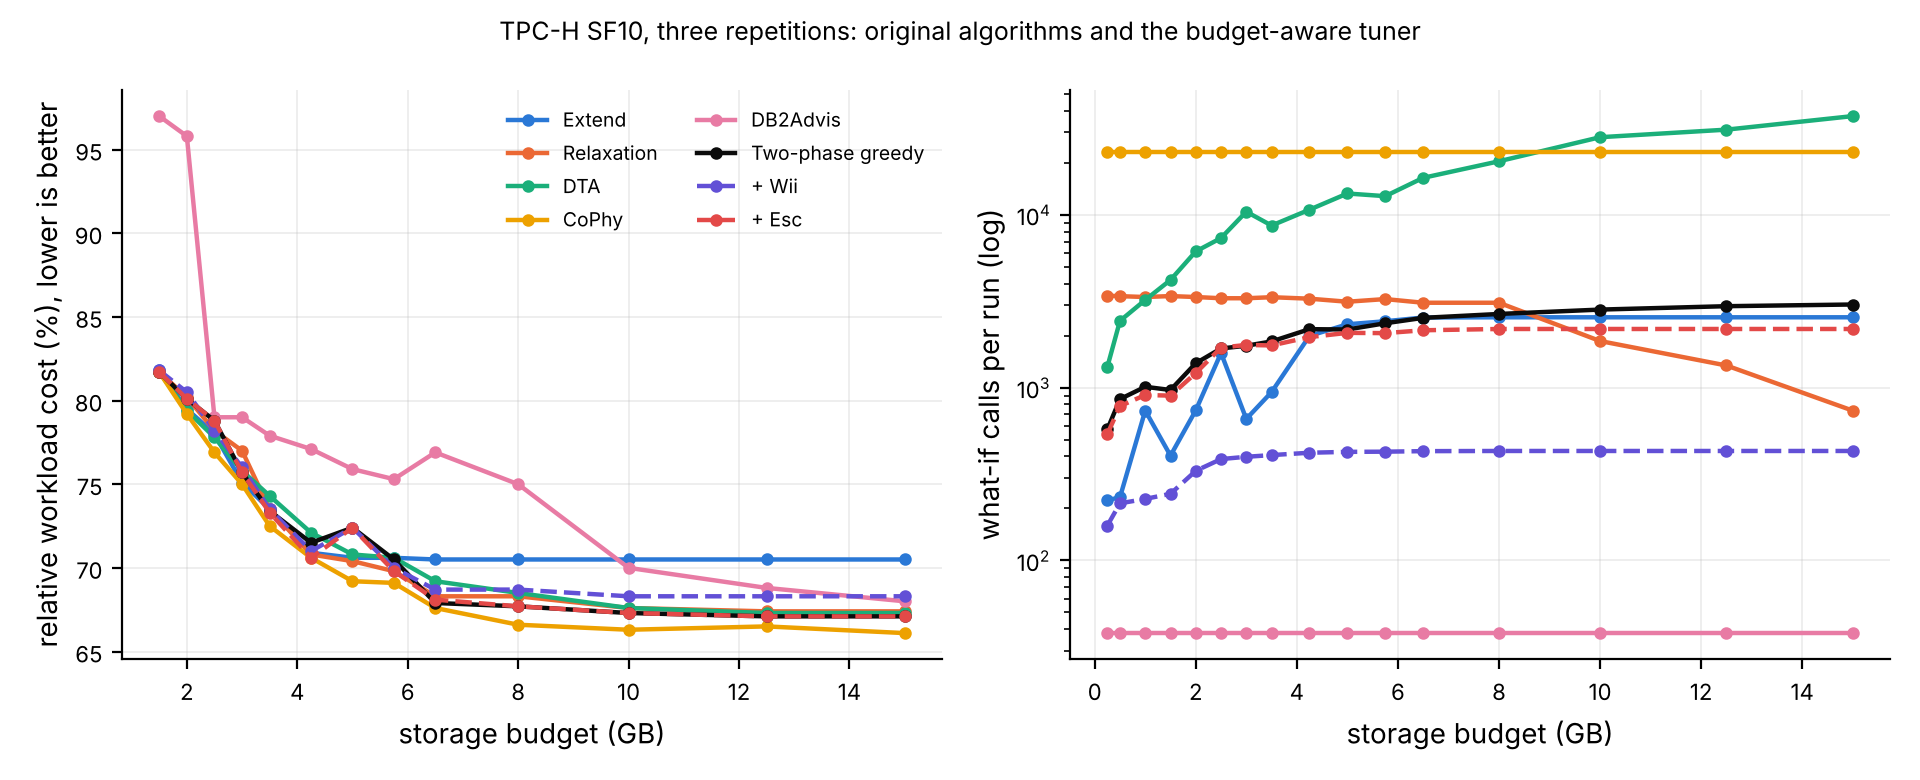
\includegraphics[width=\textwidth]{fig_compare.png}
\caption{Relative workload cost (left, from 1.5\,GB) and what-if calls (right) against the storage budget. Dashed: Wii and Esc on top of the two-phase tuner; Wii~+~Esc coincides with Wii.}\label{fig:compare}
\end{figure}

\textbf{At 10\,GB} CoPhy is best (66.3\%) but uses 23\,066 calls. The plain two-phase tuner is 1.0 point behind it (67.3\%) with 2\,828 calls, and level with Relaxation and DTA (67.6\%), AutoAdmin (67.7\%, $K=10$). With Wii the tuner is at 68.3\% with 430 calls: 2.0 points behind CoPhy, 0.7 behind Relaxation and DTA, with 1.9\% of CoPhy's calls, 23\% of Relaxation's and 1.5\% of DTA's. It beats Extend (70.5\%), DB2Advis (70.0\%), Drop (72.2\%) and Dexter (70.7\%). Only DB2Advis uses fewer calls (38) and it is 1.7 points worse than Wii. At 15\,GB the order is the same (CoPhy 66.1, two-phase 67.1, DTA 67.3, Relaxation 67.4, Wii 68.3). Wii is about one point worse than the plain tuner from 6.5\,GB on, as in the call-budget experiments.

\textbf{At 5\,GB} the greedy variants (72.4\%) are worse than Extend, Relaxation and DTA (70.4--70.8\%) and than CoPhy (69.2\%). They are also worse than at 4.25\,GB (71.5\%, Wii 71.0\%): with more room the greedy search takes a different early index and ends up worse, which we did not investigate. Below about 4\,GB all algorithms except DB2Advis are within 2--3 points of each other.

\textbf{Esc} changes the cost of the plain tuner by at most 0.2 points while saving up to 28\% of its calls (previous section), which puts it at 2\,184 calls at 10\,GB. Caveats: the tuner uses index width 2 and the original algorithms the study's own configuration; calls are counted by different code paths (the platform's cost-request counter for the original eight, the oracle's calls for ours); the original eight and our variants come from different runs; all costs are optimizer estimates.

\section{Real execution}\label{sec:exec}
Everything above uses optimizer estimates for hypothetical indexes. For the third objective of the proposal we built the indexes selected at a 5\,000\,MB budget for real in the SF10 database and ran the 19 queries (\texttt{scripts/execute\_selected\_indexes.py}; runtime per query is the median of the timed repetitions, the analysis output reports three; a query is stopped after 5 minutes and counted as 5 minutes). The workload without indexes takes 669.9\,s. Indexes are those chosen by the first repetition of each configuration.

\begin{table}[h]\centering\small
\begin{tabular}{lrrrl}
\hline
Configuration & Indexes & Estimated & Real & Queries $>10\%$ slower\\
\hline
Extend & 6 & 28.7\% & $-7.7$\% & 10\\
Relaxation & 7 & 28.8\% & $-3.3$\% & 9\\
Two-phase greedy & 7 & 26.5\% & $+35.1$\% & 7\\
Two-phase greedy + Wii & 3 & 26.4\% & $-19.4$\% & 9\\
Two-phase greedy + Esc & 6 & 26.5\% & $-40.0$\% & 11\\
Two-phase greedy + Wii + Esc & 3 & 26.4\% & $-38.3$\% & 9\\
\hline
\end{tabular}
\caption{Improvement of the workload runtime over no indexes (positive is faster), estimated against measured, at 5\,GB.}
\end{table}

\begin{figure}[h]\centering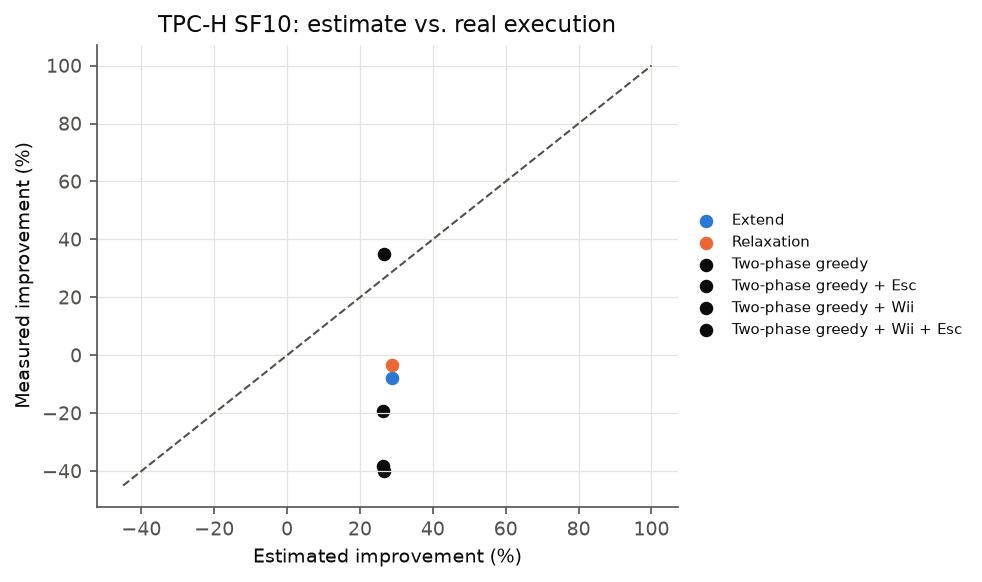
\includegraphics[width=0.8\textwidth]{fig_execution.png}\caption{Estimated against measured improvement; the dashed line is agreement.}\end{figure}

The estimates do not predict the measured result. All six configurations are estimated to improve the workload by 26--29\%, but only the plain two-phase greedy is faster in practice; the other five make the workload slower. Two-phase greedy and two-phase greedy + Esc have the same estimated improvement (26.5\%) and measured improvements 75 points apart, with index sets of 7 and 6 indexes. Queries 9 and 10 are more than 10\% slower in all six configurations, and several others (1, 4, 7, 12) in most of them. The differences between methods in the estimated tables (a few points) are much smaller than the gap between estimate and execution, so those tables do not show which method chooses better indexes in practice.

What this does not show: that Wii or Esc choose worse indexes in general. It is one budget, one selection per configuration, and 19 queries; Esc returns the configuration of its simulated greedy, built from derived costs, which can differ from the plain tuner's; timeouts are counted at 5 minutes, which hides the size of the slowdown of the slowest queries. We have not examined which indexes cause the slowdowns, nor tested possible causes (for example statistics after the indexes are built, cache state or planner settings), so we give no explanation.


\section{Discussion and limitations}\label{sec:limits}
\begin{itemize}
\item \textbf{Estimates against execution.} Section~\ref{sec:exec} is the only part that measures real runtimes, at one budget (5\,GB) with one selection per configuration. It shows that estimated improvement does not predict measured improvement, so the quality figures of Sections~\ref{sec:repro}--\ref{sec:compare} describe the optimizer's model and nothing more. We did not find out which indexes cause the slowdowns, or why.
\item \textbf{Statistics draws.} Each \texttt{ANALYZE} moves the improvement of a run by about 1 point (Wii 32.2--33.3\% over four draws). Absolute values should not be read to better than that; paired differences between methods on the same draw were stable. The assumption and gap experiments (Sections~\ref{sec:gaps} and~\ref{sec:assump}) use one draw, and the Esc results two or three.
\item \textbf{Our own implementations.} Neither Wii nor Esc has public code, and we had no reference implementation to compare against. The paper's numbers are not reproduced: Esc saves up to 28\% of the calls here against about 60\% reported for SQL Server, and Wii's 86\% saving was measured on one workload. Of the Esc paper, only Esc-B is implemented; Esc-I, the rate-based filter and the MCTS variants are not.
\item \textbf{Esc additions are ours.} The storage-aware bound and the clamp are not in the paper. The bound is valid by construction (checked by unit tests and on synthetic data). The clamp assumes monotone costs, which PostgreSQL does not guarantee (we saw $\eta_U<\eta_L$), so it is a heuristic. We did not measure on TPC-H how much of Esc's stopping the storage-aware bound is responsible for; the ablation configuration exists (\texttt{configs/tpch\_sf10\_esc\_ablation.json}) but its results are not part of this report.
\item \textbf{Wii was never limited by its budget.} Wii used at most 437 calls, so the budgets of the sweep did not constrain it; a sweep at 50--400 calls, and Esc under a call budget, are open. The greedy variants dip at 5\,GB (72.4\% against 71.5\% at 4.25\,GB), which we did not investigate.
\item \textbf{One workload, one DBMS.} Only TPC-H at SF10 on PostgreSQL; TPC-DS and JOB are not run. A teammate's run with \texttt{max\_parallel\_workers\_per\_gather}=8 gave a lower cost scale and, as reported to us, the same qualitative patterns; we report only the default-settings results.
\end{itemize}

\section{Conclusion}
The reproduction supports the original study's main findings on PostgreSQL 18: quality is determined mainly by whether a few key indexes fit in the budget, most algorithms converge to similar estimated cost, and they differ mostly in run time and what-if calls. In estimated terms, Wii keeps most of the tuner's quality with a small fraction of its calls, and Esc saves calls under a storage budget once its bound accounts for storage, but it gives nothing on top of Wii. The real-execution check is a reminder that the estimates are the weak point: five of the six configurations we executed made the workload slower. The next steps that would matter most are executing more budgets and several selections per configuration, finding the indexes behind the slowdowns, the Wii sweep at small call budgets and the Esc ablation on TPC-H.

\section*{Reproducibility}\begingroup\raggedright
Repository \texttt{RameezWahid/magic-mirror-revisited}: reproduction on branch \texttt{sf10-arijit} (results in \texttt{benchmark\_results/tpch\_sf10\_paper\_pg18.7}, CoPhy width 2 in \texttt{tpch\_sf10\_cophy\_w2\_pg18.7}); two-phase greedy and Wii in \texttt{selection/budget\_aware.py} and \texttt{selection/algorithms/two\_phase\_greedy\_algorithm.py}; Esc on branch \texttt{esc-arijit} (\texttt{selection/esc.py}, \texttt{tests/test\_esc.py}, 10 unit tests); storage-limited runs with \texttt{configs/tpch\_sf10\_new\_algos.json} through \texttt{scripts/run\_repetitions.sh} and \texttt{scripts/analyze\_results.py}; real execution with \texttt{scripts/execute\_selected\_indexes.py} (results in \texttt{benchmark\_results/execution/tpch\_sf10\_pg18.6.csv}); the raw statistics-draw runs of Sections~\ref{sec:setup}--\ref{sec:esc} in \texttt{out/*/runs.jsonl}. Environment: PostgreSQL 18.7, HypoPG 1.4.5, Dexter 0.6.3, gurobipy 13, PuLP 3 (PuLP 4 is incompatible with the CoPhy code).

\endgroup
\section*{References}
\begin{enumerate}\small
\item J.\ Kossmann, S.\ Halfpap, M.\ Jankrift, R.\ Schlosser. Magic Mirror in My Hand, Which Is the Best in the Land? An Experimental Evaluation of Index Selection Algorithms. PVLDB 13(11), 2020.
\item S.\ Halfpap et al. Looking Deeply into the Magic Mirror. PVLDB 17, 2024 (demonstration; platform used here).
\item X.\ Wang, W.\ Wu, C.\ Wang, V.\ Narasayya, S.\ Chaudhuri. Wii: Dynamic Budget Reallocation In Index Tuning. SIGMOD 2024 (PACMMOD 2(3)).
\item X.\ Wang, W.\ Wu, V.\ Narasayya, S.\ Chaudhuri. Esc: An Early-Stopping Checker for Budget-aware Index Tuning. PVLDB 18(5), 2025.
\end{enumerate}
\end{document}
